%
%  untitled
%
%  Created by Stephan Gabler on 2010-06-16.
%  Copyright (c) 2010 __MyCompanyName__. All rights reserved.
%
\documentclass[]{article}

% Use utf-8 encoding for foreign characters
\usepackage[utf8]{inputenc}

% Setup for fullpage use
\usepackage{fullpage}

% Uncomment some of the following if you use the features
%
% Running Headers and footers
%\usepackage{fancyhdr}

% Multipart figures
%\usepackage{subfigure}

% More symbols
%\usepackage{amsmath}
%\usepackage{amssymb}
%\usepackage{latexsym}

% Surround parts of graphics with box
\usepackage{boxedminipage}

% Package for including code in the document
\usepackage{listings}

% If you want to generate a toc for each chapter (use with book)
\usepackage{minitoc}

% This is now the recommended way for checking for PDFLaTeX:
\usepackage{ifpdf}

%\newif\ifpdf
%\ifx\pdfoutput\undefined
%\pdffalse % we are not running PDFLaTeX
%\else
%\pdfoutput=1 % we are running PDFLaTeX
%\pdftrue
%\fi

\ifpdf
\usepackage[pdftex]{graphicx}
\else
\usepackage{graphicx}
\fi
\title{Machine Intelligence II \\ Exercise 6 (ICA)}
\author{Group 1 \\ Tiziano, Rafael and Stephan}

\date{\today}

\begin{document}

\ifpdf
\DeclareGraphicsExtensions{.pdf, .jpg, .tif}
\else
\DeclareGraphicsExtensions{.eps, .jpg}
\fi

\maketitle

\section{Results}

After applying the mixing transformation $A$ the mixed signal and the sources are still significantly correlated.
However after permuting the samples this correlation drops to zero. 
\par We use the permuted signal to estimate the 
un-mixing matrix $W$ which we use to recover the original sources. This shows that ICA does not rely on the order in which the samples are presented.
As expected, the correlation of the recovered sources with the original ones is high and close to 1.
For example we obtain these correlation values:
correlation signal vs. sources: 0.79999\\
correlation signal (permuted) vs. sources: -0.0040099\\
correlation sources vs. rec. sources: 0.9967\\
\par
Figure 1 shows that the ICA algorithm can recover the sources in a different order and with an arbitrary scaling factor.
In order to compute the right correlations at the end we thus need to figure out the order in which the sources have been reconstructed.

\begin{figure}[h!]
	\centering
		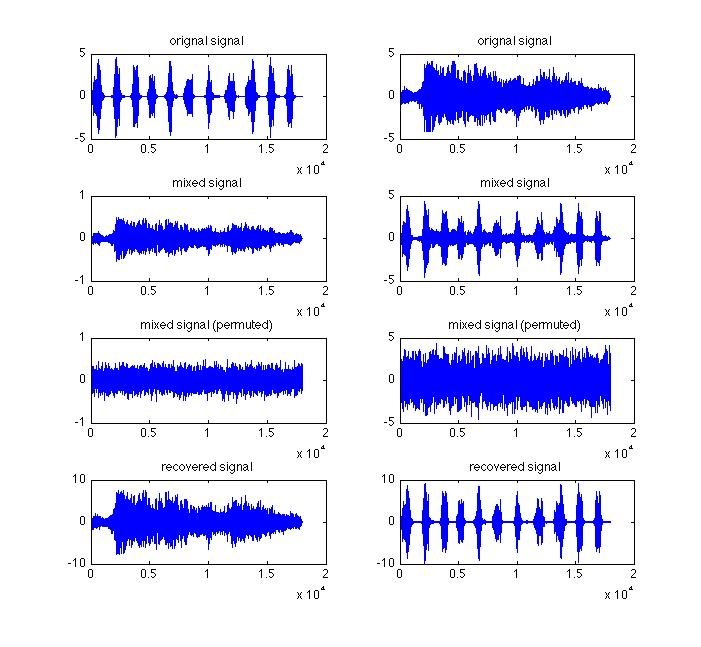
\includegraphics[width=1\textwidth]{sound_plot.jpg}
	\caption{Plots of the signals}
	\label{sg:fig:sound_plot}
\end{figure}

\end{document}
